\documentclass[letterpaper]{article}
\usepackage{natbib,alife13}

\title{Aracna: An Open-Source Quadruped Platform for Evolutionary Robotics}
\author{Sara Lohmann, Eric Gold, Jason Yosinski, Jeremy Blum \and Hod Lipson \\
\mbox{}\\
Cornell University, 239 Upson Hall, Ithaca, NY 14853 \\
\texttt{sml253@cornell.edu}}



\begin{document}
\maketitle

\begin{abstract}
We describe a new, quadruped robot platform, Aracna,
which requires non-intuitive motor commands in order to locomote and thus provides an interesting challenge for gait learning algorithms, such as those frequently developed in the Evolutionary Computation and Artificial Life communities. Aracna is an open-source hardware project composed of off-the-shelf and 3D-printed parts, enabling other research teams to modify its design according to their scientific needs. Aracna was designed to avoid the Achilles Heel of a previous quadruped robot platform, whose legs were so heavy that the motors could not reliably execute the commands sent to them. Aracna minimizes leg inertia to avoid this problem by having all motors located in the body core instead of on the legs.  Specifically, each of the four legs has two joints separately controlled by separate four-bar linkage
mechanisms that drive the pitch of the hip joint and knee joint remotely from motors in the robot's core. 
%The eight kinematic degrees of freedom in Aracna are controlled by its eight servos. 
This novel design causes unconventional kinematics, however, creating an opportunity for gait-learning algorithms, which excel in counter-intuitive design spaces where human engineers tend to underperform.  Because it is low-cost, flexible, kinematically interesting, and and improvement over a previous design, Aracna provides a useful new hardware platform for testing algorithms that automatically generate robotic behaviors. 
\end{abstract}



\section{Introduction}

There is a long history in the Artificial Life and Evolutionary Robotics community of automatically generating behaviors for robots~\citep{nolfi2000evolutionary, pfeifer2007body, sims1994evolving, hornby2005autonomous, lipson2000automatic}. Much work has focused on evolving gaits for legged robots~\citep{clune2009evolving, clune2011performance, hornby2005autonomous, hornby2003generative, kodjabachian1998evolution, Koos2012, bongard2006resilient, yosinski2011gaits, gallagher1996application}. While some of this previous work involved evolution directly on a physical robot~\citep{yosinski2011gaits, zykov2004evolving}, more often a gait was evolved in simulation and then transferred to the physical robot~\citep{lipson2006evolutionary, Koos2012, hornby2005autonomous, bongard2006resilient}. Many of these studies report that evolutionary algorithms produced gaits that outperformed those designed by a human engineer~\citep{yosinski2011gaits, hornby2005autonomous}, which is not surprising given that evolutionary algorithms routinely create solutions that are superior to manually created solutions~\citep{koza2003genetic}. 

\begin{figure}[t]
\begin{center}
%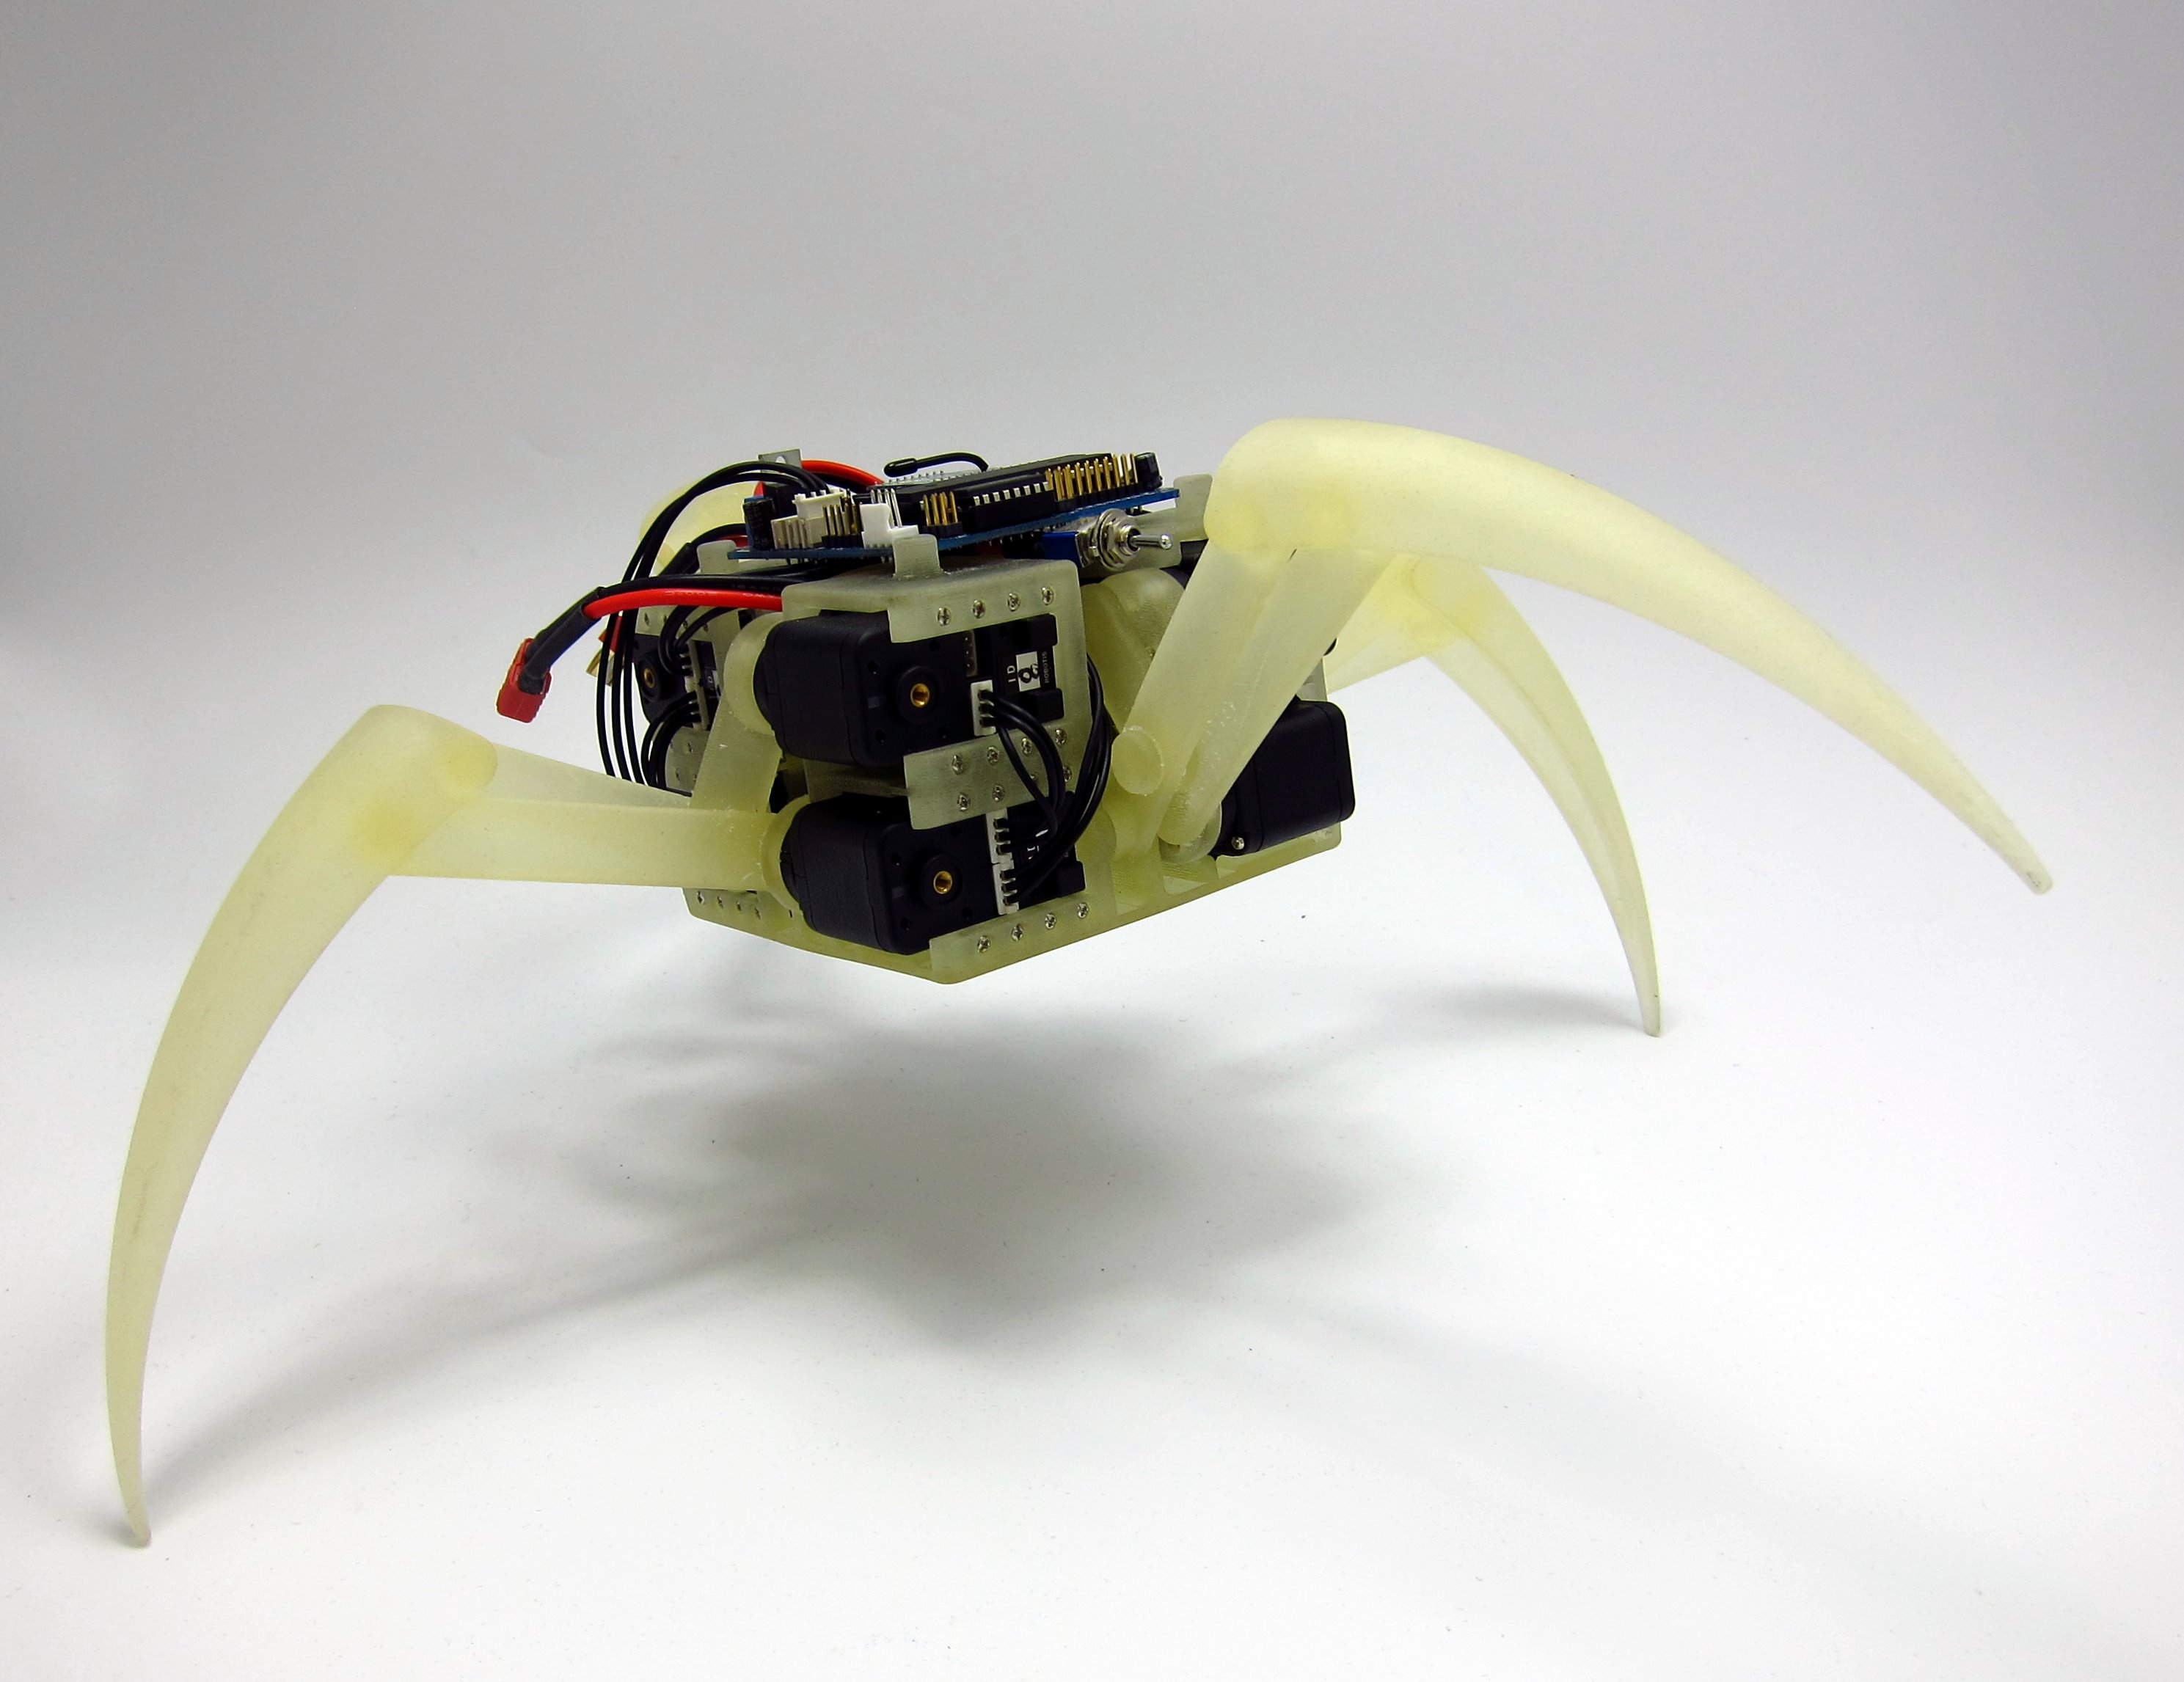
\includegraphics[width=.45\textwidth]{fig1.jpg}
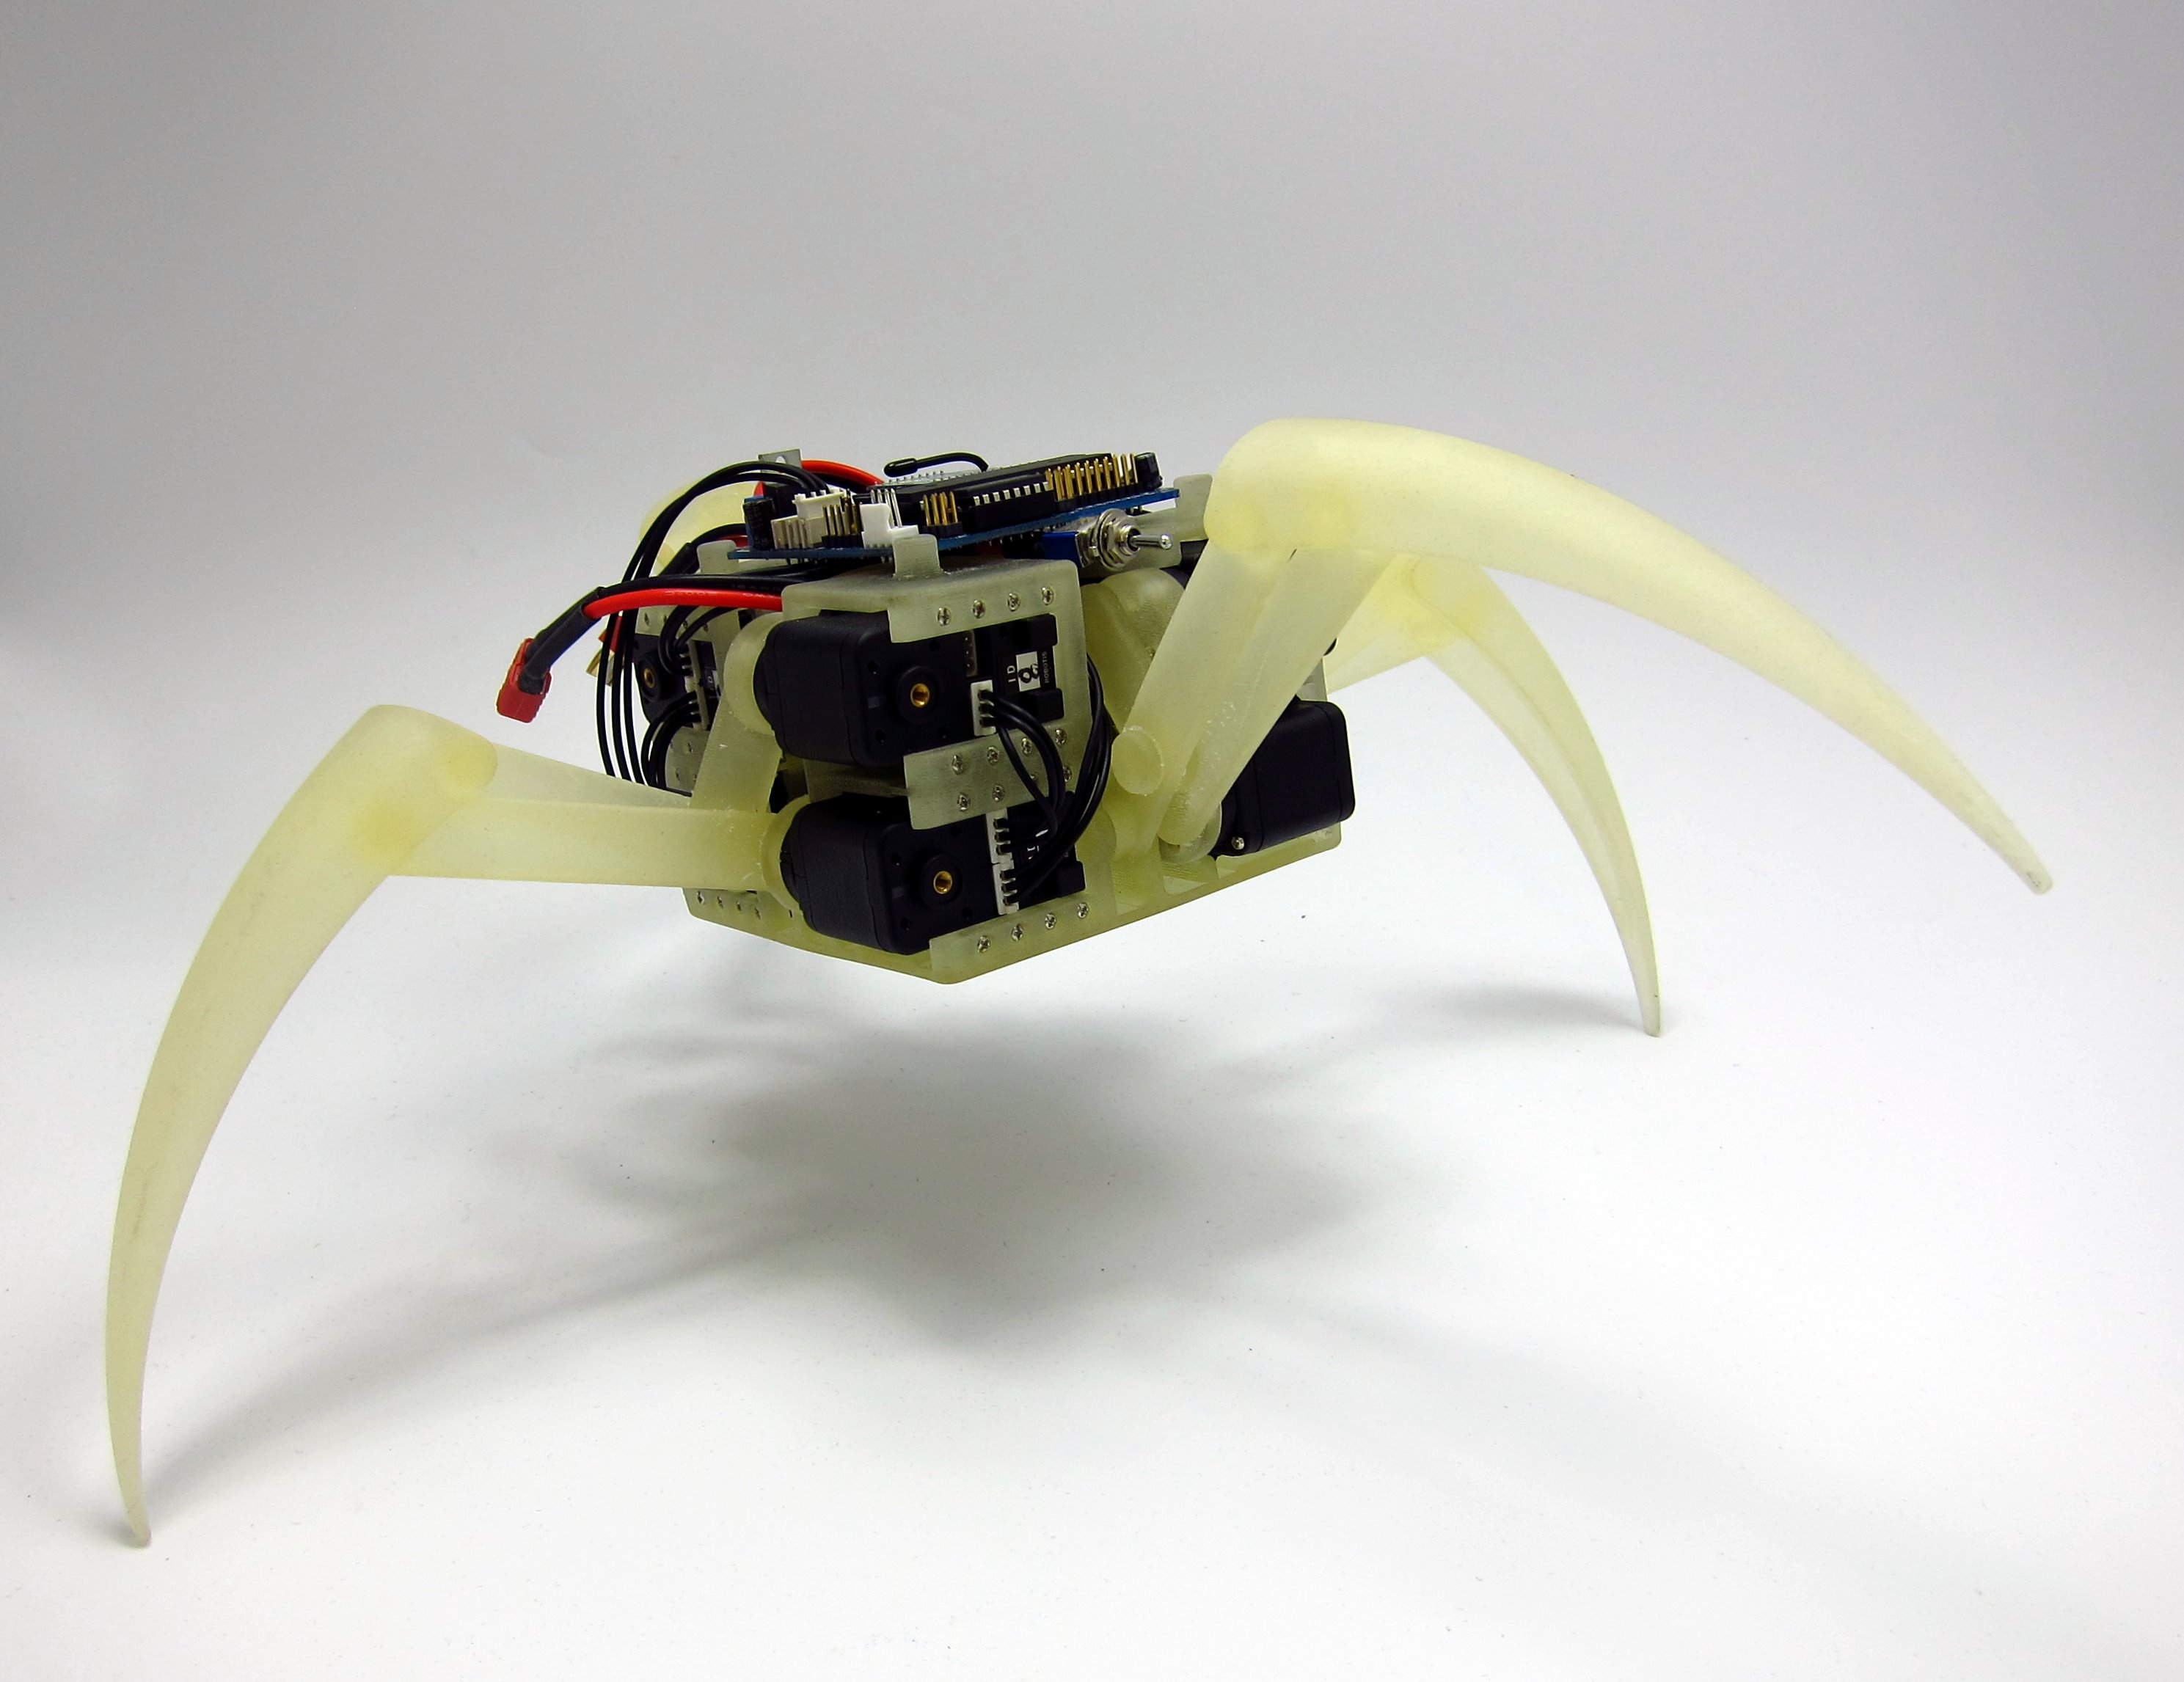
\includegraphics[width=\columnwidth]{fig1.jpg}
\caption{Aracna: an open-sourced quadruped robot platform. All
  instructions and downloads are publicly available at
  http://creativemachines.cornell.edu/aracna .}
\label{fig1}
\end{center}
\end{figure}

The results just mentioned suggest that evolutionary algorithms are a promising approach for generating gaits and other behaviors for physical robots. Despite this promise, the field remains small, partly because robots are expensive and they are difficult to modify. Access to cheap, customizable robots could increase the number of researchers able to participate in the field. Moreover, in nearly all of the papers mentioned previously, the robots were custom-made, preventing teams at other universities from reproducing the results of other groups and or testing new algorithms on a robotic platform used in a previous study. That, in turn, slows the progress of science because it is difficult to interpret whether the variance in results between different studies was due to the algorithms used or the robotic platform those algorithms were tested on.  

Some robot platforms are emerging, but they tend to be wheeled robots without complex kinematics, such as the ePuck~\citep{mondada2009puck}. Wheeled robots are interesting testbeds for many robotic behaviors, but they do not allow gait evolution and are unable to traverse rugged terrains. Legged robotic platforms exist, but they tend to be extremely expensive, such as the Aldebaran Nao, which costs more than \$10,000 USD. Another drawback to these commercial platforms is that it is hard, if not impossible, to modify the hardware design because they are not open-source hardware projects, and do not take advantage of off-the-shelf components and 3D printing, meaning that complex manufacturing tools are required to manufacture newly designed parts. 

In this paper we address these needs by introducing \emph{Aracna}, a low-cost, open-source hardware, easily customizable robot platform with non-intuitive walking
kinematics~(Figure 1). Aracna is the third quadruped robot developed for evolutionary learning algorithms by the Creative Machines Lab at Cornell University~\citep{bongard2006resilient, yosinski2011gaits}. Like the most recent of the two previous designs, called QuadraTot~\citep{yosinski2011gaits}, the body of Aracna is 3D printed and the STL files are available online,
%TODO: INSERT LINK
meaning that other researchers can easily customize the body's design. As in the both previous designs, each leg has a hip and knee joint controlled by two actuators. The original Creative
Machines Lab quadruped robot favored starfish-like movements~\citep{bongard2006resilient}. The second quadruped robot --- QuadraTot ---
developed spider-like movements, but was found to be limited by its
weight, such that the motors would overheat and timeout when trying to execute many commands~\citep{yosinski2011gaits, Glette2012Evolution}. We designed Aracna to be able to produce fast, spider-like movements, yet be lightweight enough that the motors would not overheat. We also designed Aracna to be inexpensive: as described below, its overall price is under \$1,400  USD. In the following sections we describe the Aracna platform in more detail. 




\section{Overall Hardware Design}

\begin{figure}[t]
\begin{center}
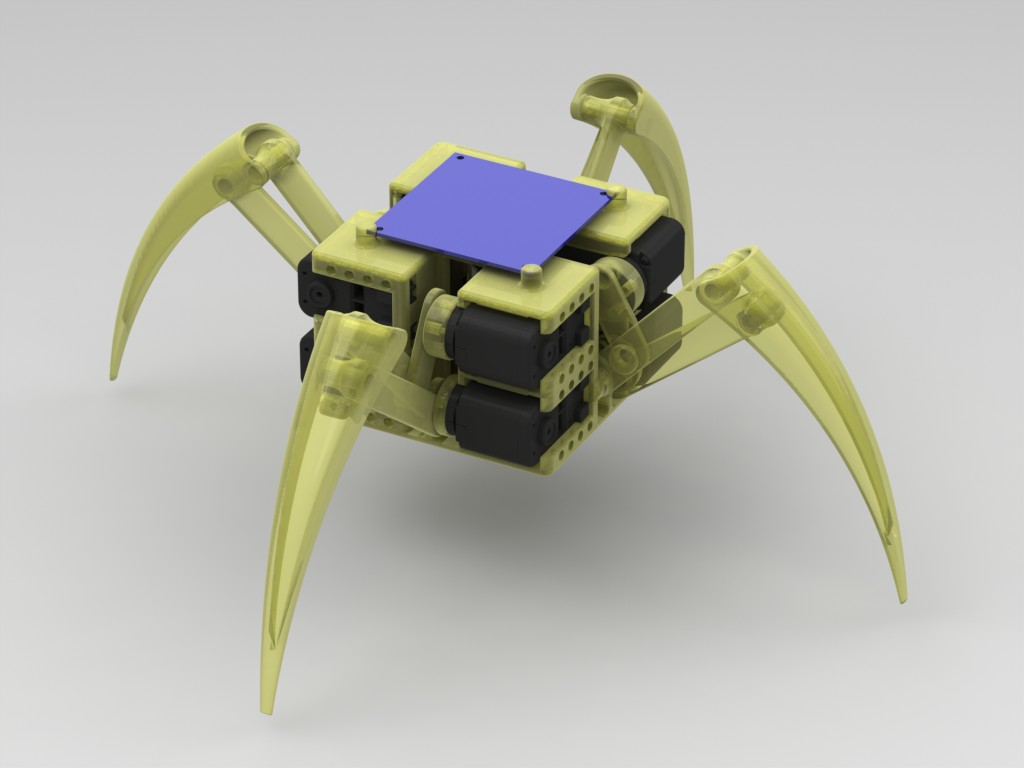
\includegraphics[width=\columnwidth]{fig5.jpg}
\caption{A rendered CAD model of Aracna. Note the lack of heavy servos on the legs themselves, which are instead controlled via four-bar linkages by servos in the robot's core.}
\label{cadModelOfRobot}
\end{center}
\end{figure}



%\begin{figure}[t]
%\begin{center}
%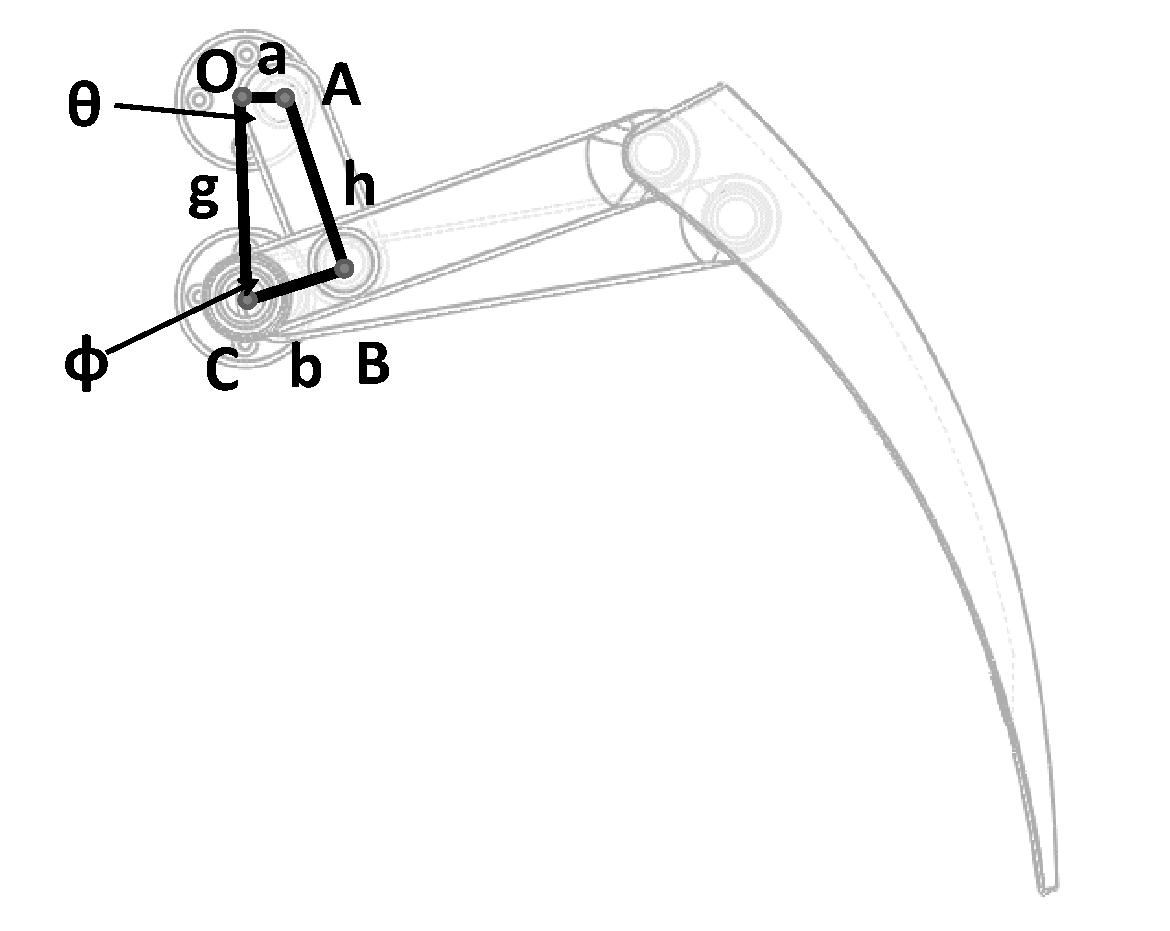
\includegraphics[width=2.25in,angle=0]{fig4.pdf}
%\caption{Crank-rocker four-bar linkage controlling flexion/extension of the hip joint.}
%\label{fig4}
%\end{center}
%\end{figure}

The hardware of Aracna was designed to improve upon the previous Creative Machines Lab
quadruped robots~\citep{bongard2006resilient, yosinski2011gaits}, while still qualitatively resembling those robots. Aracna is similar in that it has a body and four legs, with each leg having two joints that can pitch forward and back like knees~(Figure~\ref{cadModelOfRobot}). 

One change was to constrain the movement of the
joints toward the goal of creating faster, spider-like movements. To
prevent starfish-like movements and instead encourage a walking gait with the robot body permanently off the ground, the legs were constrained such that they cannot straighten out and the knee cannot hyperextend. 

Another change was to reduce the both the overall weight of the robot and the weight of each leg. Two previous studies that used the QuadraTot robot report that the motors quickly wore out and could not reliably execute the commands sent to them, likely because of both the overall weight of the QuadraTot and the fact that housing servos on the legs made them heavy~\citep{bongard2006resilient, yosinski2011gaits}. The weight of the robot's core was reduced in a number of ways. 

Initially, we eliminated the QuadraTot's fit-PC, an onboard Linux computer weighing 370g, and replaced it with an on-board ArbotiX microcontroller that weights only 47g. As a result, the main processing occurs on an external computer and commands are sent to Aracna wirelessly. This change, of course, comes of the cost of the robot being truly autonomous. Wireless communication between the external control computer
and the ArbotiX  microcontroller occurs over wireless XBee.

A second means of eliminating weight involved switching to a lighter battery. The QuadraTot had two 12V lithium-ion battery packs that weighted 140g each for a total of 280g. Aracna has a single lithium-polymer 11.1V battery that weighs 122 g. INSERT SENTENCE ON THE COST/PENALTY OF USING THE SMALLER BATTERY.   

A major modification, targeted at reducing the weight of legs, was the use of two four-bar mechanisms to drive the joints in each
leg. This mechanism causes the controlled joint to move at a fraction
of the output angle of the actuator, giving the motor a relatively
larger mechanical advantage over the position of each leg.
Figure~\ref{crankRocker} shows the crank-rocker system, where the input crank
is actuated by a servo and the rocker is the leg. This
configuration allows the servo motors to be contained in the robot core, reducing both the inertia and mass of each leg. The weight of an Aracna leg is 105g compared to the 217g for a QuadraTot leg.  

Combined, these changes to minimize weight led to a 31.4 percent reduction in weight of the robot. The QuadraTot weighs 1.88kg whereas Aracna weighs 1.29kg.

A final change was to upgrade the power of the servo motors in order to increase the ability of the robot to strike whichever configurations are specified by the learning algorithms. Specifically, we upgraded from Dynamixel AX 12+ motors to AX-18A motors, which have a higher stall torque (1.8Nm vs. 1.5Nm at 12V), a higher stall current (2.2A vs 1.5A), and a higher no load speed (97 vs. 59 RPM).


\begin{figure}[t]
\begin{center}
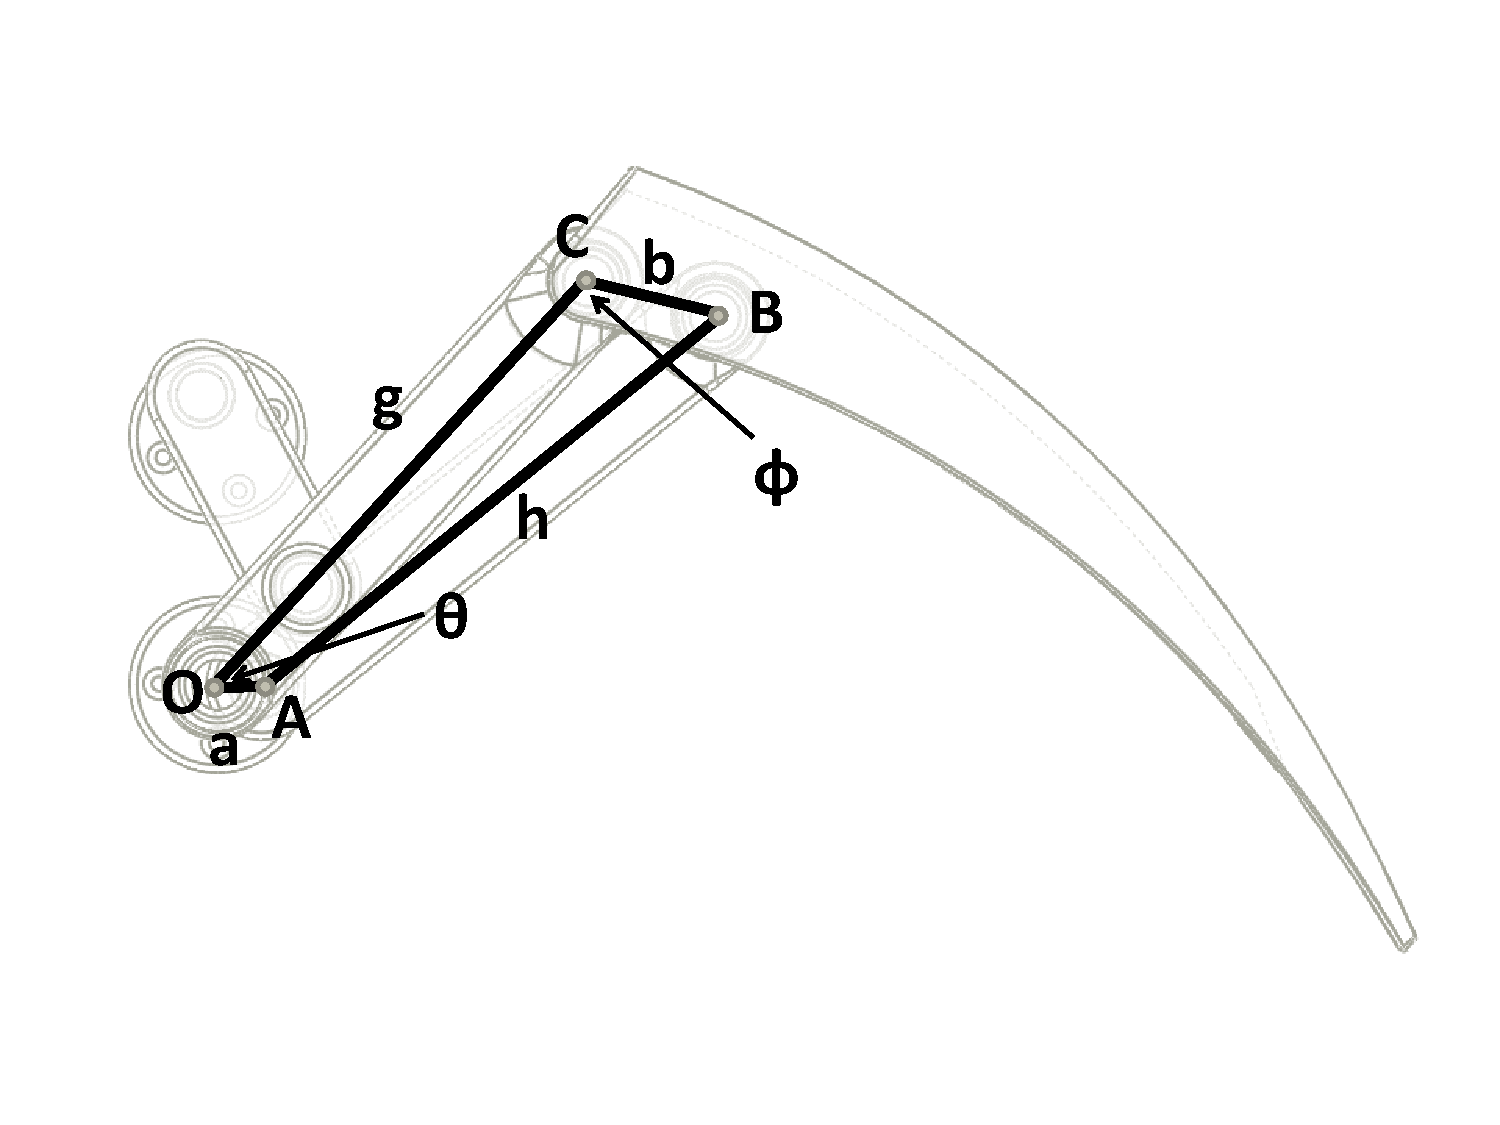
\includegraphics[width=.23\textwidth]{fig3.pdf}
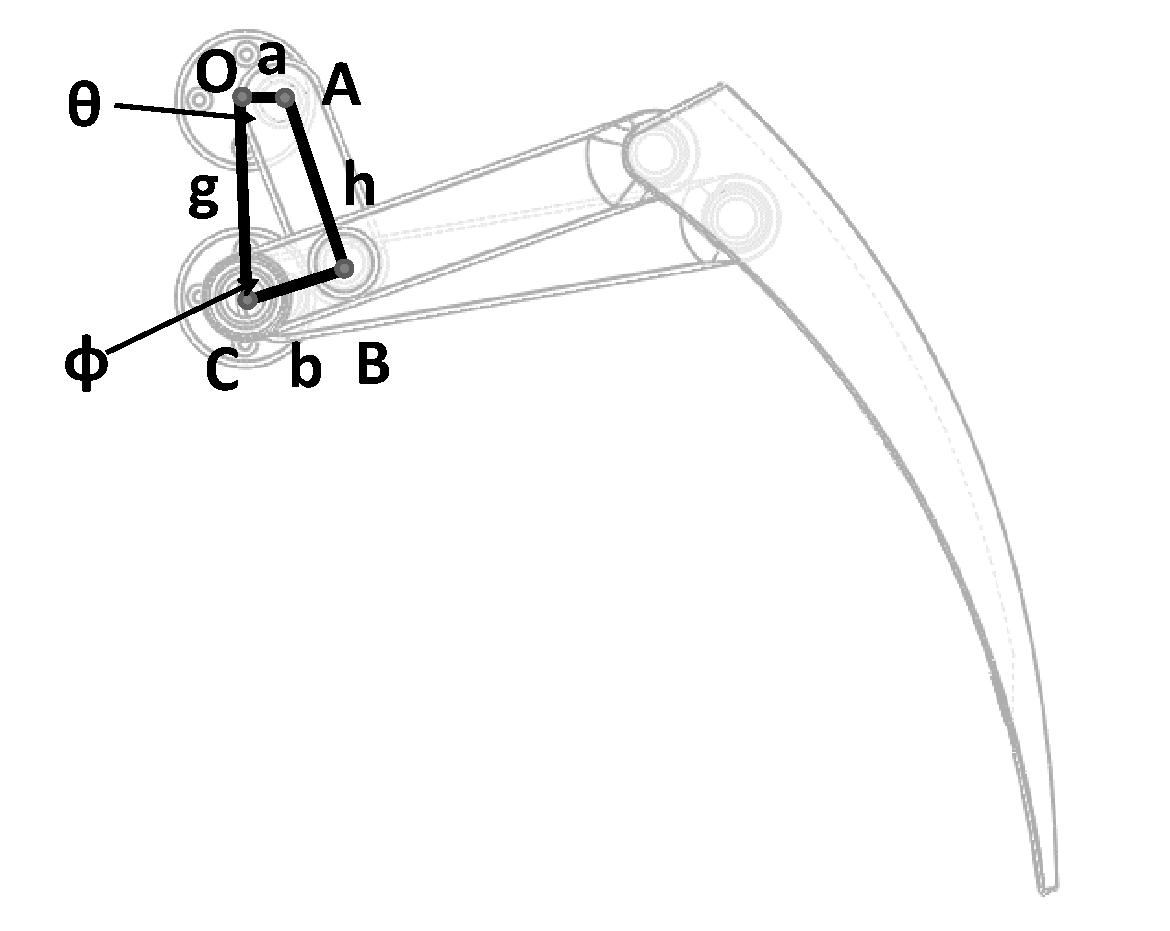
\includegraphics[width=.23\textwidth]{fig4.pdf}
\caption{Crank-rocker four-bar linkage controlling flexion/extension of
  the knee and hip joints. In both cases above, the input crank (link
  OA) is actuated by a servo, the rocker is the leg (link CB), and the
  fixed link is OC.}
\label{crankRocker}
\end{center}
\end{figure}


\section{3D Printed Body}

The body of Arcana takes advantage of 3D printing technology, also known as additive manufacturing, which generates physical objects from digital designs by building them up layer by layer~\citep{gibson2009additive, lipson2010factory}. The use of 3D printing means that other Aracna users can easily make copies of Aracna, either by having access to a 3D printer or via online 3D printing services such as Shapeways.com. Either option requires the 3D design files in the stereolithography (STL) format, which we are publishing in the online support material for this paper~\citep{WEB}. Moreover, to catalyze innovation in this open-source hardware project, we are also providing the source files for the SolidWorks computer-aided-design program, to enable others to modify the design. It should thus be easy for future Aracna users to improve or alter the design and quickly obtain a physical instantiation of the design. Importantly, the use of 3D printing eliminates the need to know how to machine parts, allowing many more researchers to participate in using physical robot morphologies that they design themselves. These ideas are in line with a broader trend toward enabling non-technical users to design and manufacture physical objects~\citep{clune2011objects, clune2011endless, lipson2010factory}.

An initial version of Aracna was designed to be printed in one piece~(Figure~\ref{notYetCleanedOnePieceRobot}). However, if one part of the robot became damaged, an entire new robot had to be reprinted, which took over 26 hours and costs roughly \$355 USD on an Objet Connex500 printer. To make repairing the robot easier, cheaper, and quicker, Aracna was redesigned to be modular. It consists of 15 pieces--four legs and the core--that can be separately 3D printed~(Figure~\ref{notYetCleanedMulitPieceRobot}). Printing a leg takes 3.3 hours and costs roughly \$64 USD. Printing the core takes 3 hours and costs \$101 USD. All 15 Aracna pieces can still be printed as one print job, with an overall time of approximately 10 hours and cost of \$308. These figures are based on Aracna's use of  approximately 967g of model material and 746g of support material, and current material costs of 4.5g per USD and 8g per USD for rigid and support material, respectively. This cost estimate is variable depending on the type of material used. The print times are estimates calculated by the Objet's software and are meant to be used as a relative comparison of print times. Table~\ref{tab:cost} outlines the total estimated cost of Aracna, which is just under \$1,400, including its off-the-shelf electronic components. 


\begin{figure}[t]
\begin{center}
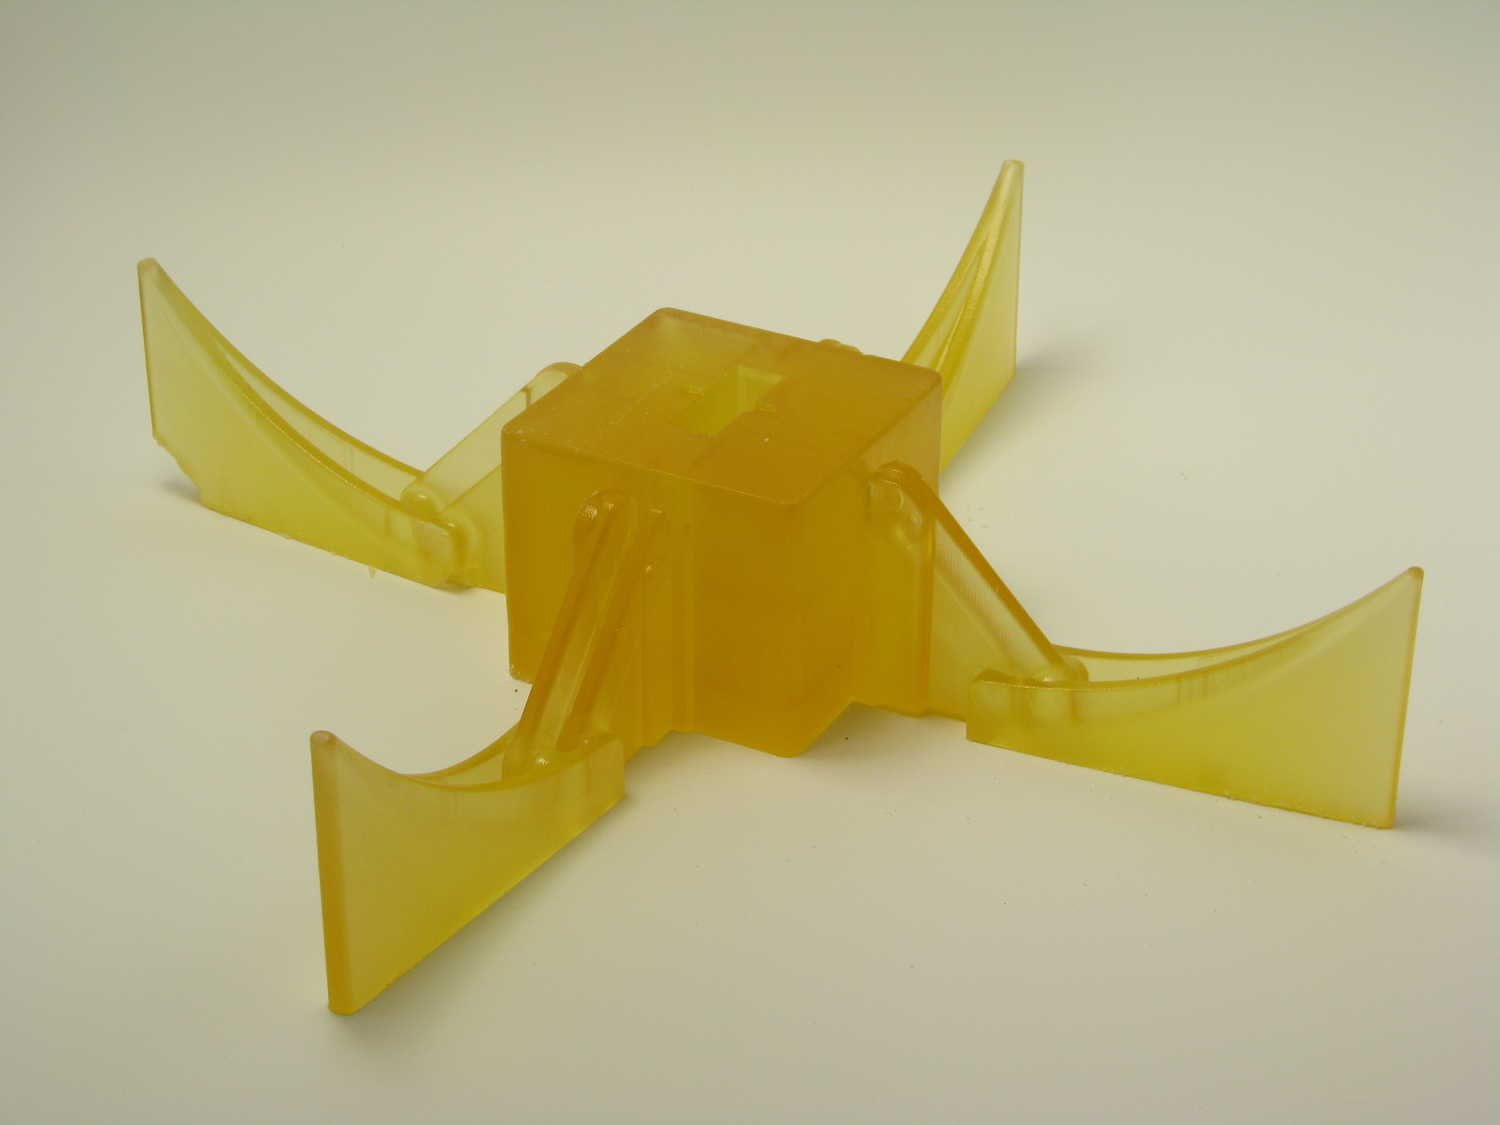
\includegraphics[width=.37\textwidth]{fig2.jpg}
\caption{A draft version of Aracna that was printed in one piece. This non-modular design proved expensive to maintain if part of the robot was damaged, and was replaced in a later version with a modular design. This image is of the printed body with support material still present.}
\label{notYetCleanedOnePieceRobot}
\end{center}
\end{figure}

\begin{figure}[t]
\begin{center}
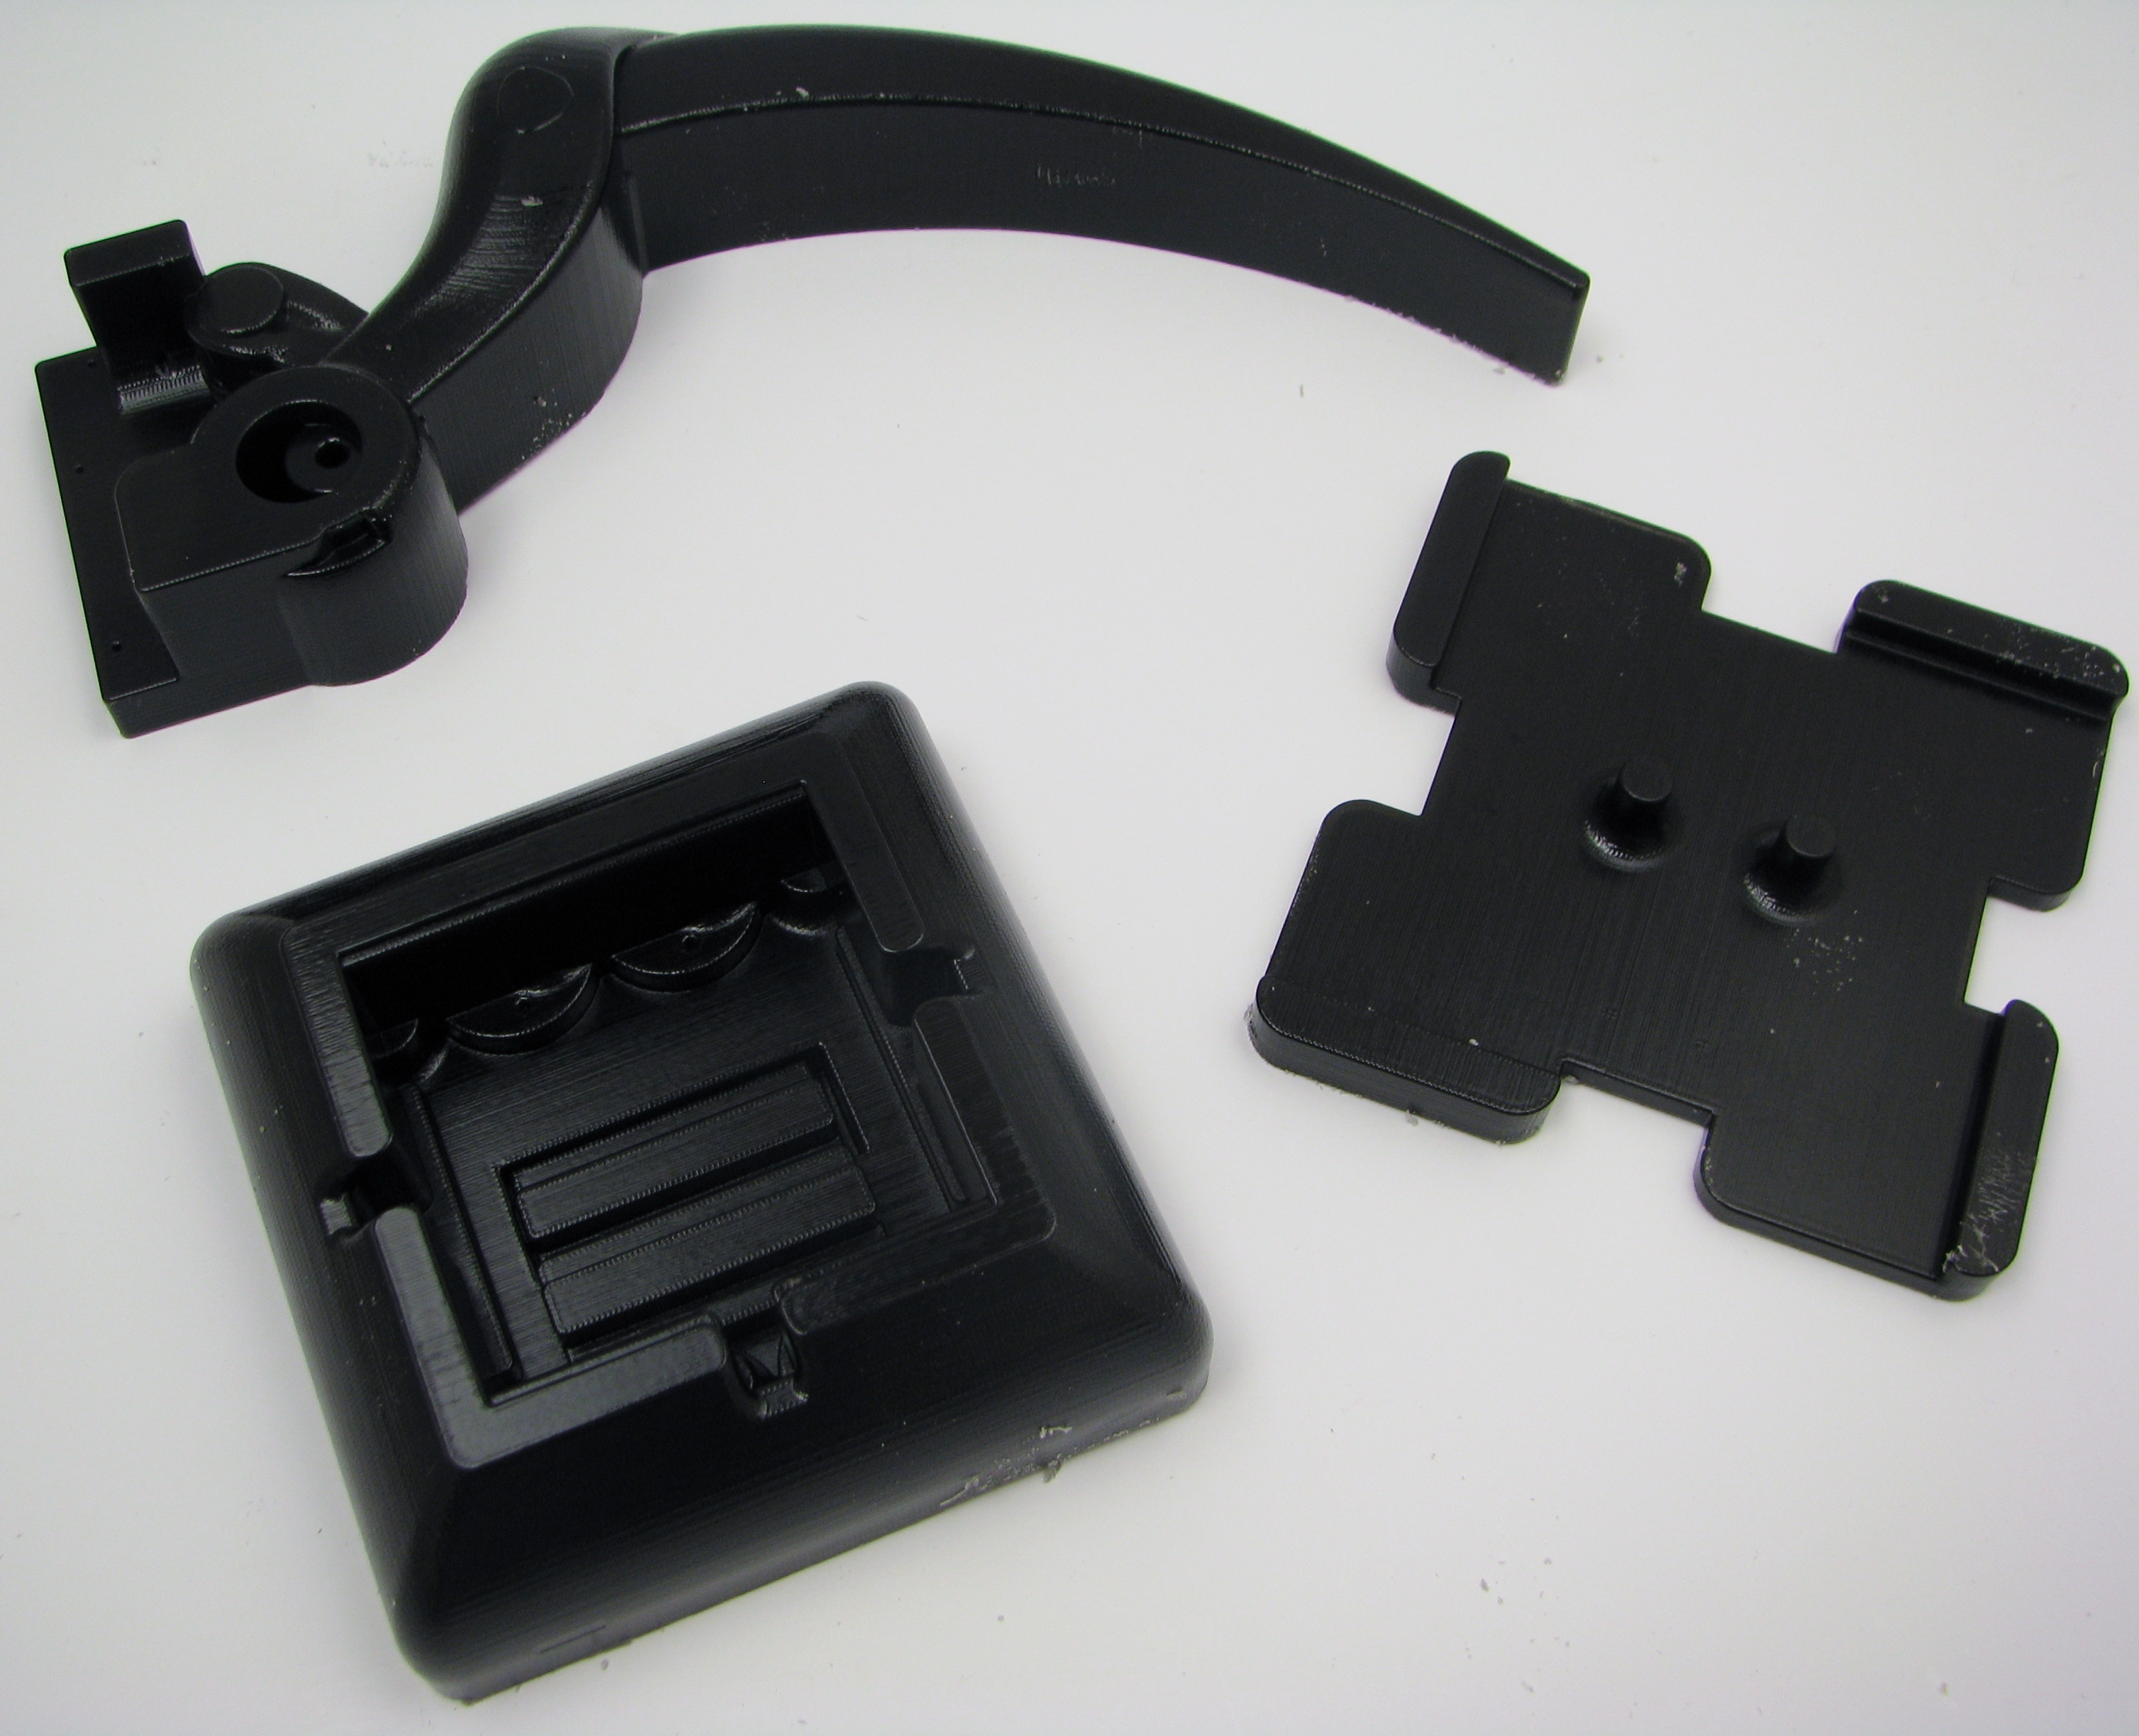
\includegraphics[width=.37\textwidth]{fig6.jpg}
\caption{A final version of Aracna printed in multiple pieces.The body is printed as two pieces, with 9 smaller parts within the top piece to reduce support material and print time. These parts can be printed individually if replacements are necessary. The body consists of a total of 11 parts. This image shows a set of 12 printed parts (the complete body and a single leg) with support material still present.}
\label{notYetCleanedMulitPieceRobot}
\end{center}
\end{figure}


\begin{table}[h]
\center{
\begin{tabular}{|c|c|}
\hline
Part & Cost\\
\hline\hline
3D Print Materials & \$308\\
ArbotiX Robocontroller Kit & \$189\\
Dynamixel AX-18A Robot Actuator (x8) & \$721\\
3S 11.1V 2000mAh Pro Lite LiPo Battery & \$73\\
LiPo Battery Balance Charger Kit & \$70\\
Cables, Connectors, Misc & \$28\\
\hline\hline
\bf Total & \bf \$1389\\
 \hline
\end{tabular}
}
\vskip 0.25cm
\caption{Estimated total cost. The cost of components and printing material reflect market prices from March 2012. A complete parts list is on our website \citep{WEB}.}
\label{tab:cost}
\end{table}


\section{Control}

In addition to reducing the weight of the legs, the four-bar
mechanisms also satisfied the design goal of making a robot that had
non-traditional movements. Unusual kinematics make for a more effective evolutionary robotics test platform, since evolutionary algorithms are most helpful in domains that humans find hard to program solutions for. The reason Aracna's kinematics are counter-intuitive is because there is a complicated mapping between each servo's output and the movement of the joint controlled by that servo~(Figure~INSERTjointAnglesAsAFunctionOfServoPositions). INSERT-OTHER-REASONS-THE-KINEMATICS-ARE-STRANGE. 

The range of motion for the hip joint is INSERT degrees and that of the knee joint is INSERT degrees~(Figure~INSERT). The range of the knee joint technically depends on the position of the hip joint, but the effect is slight enough (less than INSERT) degrees, that it can be effectively ignored. 

There are two different ways to encode movements for Aracna, increasing its flexibility as a testing platform. The first method is to specify a sequence of positions over time for all eight servos. In this method the joint angles would be determined as shown in Figure~INSERTjointAnglesAsAFunctionOfServoPositions). The second method is to set the speed of each servo (and possibly its initial position). This method is possible because with the four bar mechanism a servo constantly rotating in one direction will move the joint back and forth between its minimum and maximum opening angle. This latter method provides a much smaller search space and would encourage regular gaits, which have been shown to be beneficial when evolving gaits for legged robots~\citep{clune2011performance, hornby2005autonomous}. 


\section{Software}

The software, which is also open-source and freely available~\citep{WEB}, is written in Python and based on the
code developed for the QuadraTot platform~\citep{yosinski2011gaits}. The software translates a series of requested joint angles from the learning algorithm into servo movements. Additionally, it returns information to the learning algorithm, such as the distance traveled or the specific trajectory the robot took, so the learning algorithm can assess the quality of the gait. To provide this information, an infrared light
emitting diode (LED) was placed on the robot and a Nintendo Wii
remote was attached overhead. The software uses the combination of the two to ascertain the X, Y position of the robot. The software is interoperable with any gait or behavior learning algorithm.  

\section{Example Gaits}

Evolutionary algorithms work best when they have a gradient to follow, instead of searching for a needle in a haystack. To get a sense of how randomly-generated gaits would perform, we randomly chose a few parameters....INSERT DESCRIPTION OF WHAT YOU DID, HOW IT WORKED, AND A LINK TO THE VIDEO. 

\section{Conclusion}

I think we should wait until the rest of the paper is fleshed out before writing this. 

\section{Acknowledgements}

This work was supported by the National Science Foundation's Office of
Emerging Frontiers in Research and Innovation (grant number 0735953) and an NSF Postdoctoral Research Fellowship in Biology to Jeff Clune (DBI-1003220).


\footnotesize
\bibliographystyle{apalike}
\bibliography{references}
\end{document}

